\documentclass[11pt,a4paper]{article}
\usepackage{amsmath}
\usepackage[margin=2.2cm]{geometry}
\usepackage{graphicx}
\usepackage{xcolor}
\usepackage{listings}
\usepackage{enumitem}
\usepackage{hyperref}

% ---------- Code listing style ----------
\definecolor{codebg}{RGB}{248,248,245}
\definecolor{codeframe}{RGB}{210,208,200}
\definecolor{codekw}{RGB}{170,13,145}      % keywords (purple)
\definecolor{codestr}{RGB}{196,26,22}      % strings (red)
\definecolor{codecom}{RGB}{93,108,121}     % comments (gray-blue)
\definecolor{codenum}{RGB}{120,120,120}    % line numbers
\definecolor{codeid}{RGB}{40,40,40}        % identifiers

\lstdefinelanguage{JavaScript}{
    keywords={break,case,catch,const,continue,default,delete,do,else,
              export,extends,finally,for,function,if,import,in,instanceof,
              let,new,null,of,return,super,switch,this,throw,true,false,
              try,typeof,undefined,var,void,while,with,yield},
    keywordstyle=\color{codekw}\bfseries,
    ndkeywords={msg,flow,global,node,JSON,Math,Date,Number,String,Array,Object},
    ndkeywordstyle=\color{codekw!80!black},
    sensitive=true,
    comment=[l]{//},
    morecomment=[s]{/*}{*/},
    commentstyle=\color{codecom}\itshape,
    stringstyle=\color{codestr},
    morestring=[b]',
    morestring=[b]",
    morestring=[b]`
}

\lstset{
    language=JavaScript,
    basicstyle=\ttfamily\footnotesize\color{codeid},
    backgroundcolor=\color{codebg},
    rulecolor=\color{codeframe},
    frame=single,
    framesep=6pt,
    framerule=0.4pt,
    xleftmargin=14pt,
    xrightmargin=4pt,
    aboveskip=8pt,
    belowskip=8pt,
    numbers=left,
    numberstyle=\tiny\color{codenum},
    numbersep=8pt,
    showstringspaces=false,
    breaklines=true,
    breakatwhitespace=true,
    breakindent=12pt,
    tabsize=2,
    columns=fullflexible,
    keepspaces=true,
    captionpos=b,
    abovecaptionskip=4pt,
    belowcaptionskip=2pt
}

\setlist{nosep,leftmargin=*}

\title{IoT - Challenge 3}
\author{Raul Agolli - Team Leader \\\\ Gabriele Lorenzo Singe}
\date{April 2026}

\begin{document}

\maketitle

\section{Overview}
The Node-RED flow is composed of chains that
share state through the flow/global context and through the local MQTT
broker on \texttt{localhost:1884}.
\begin{figure}[h]
    \centering
    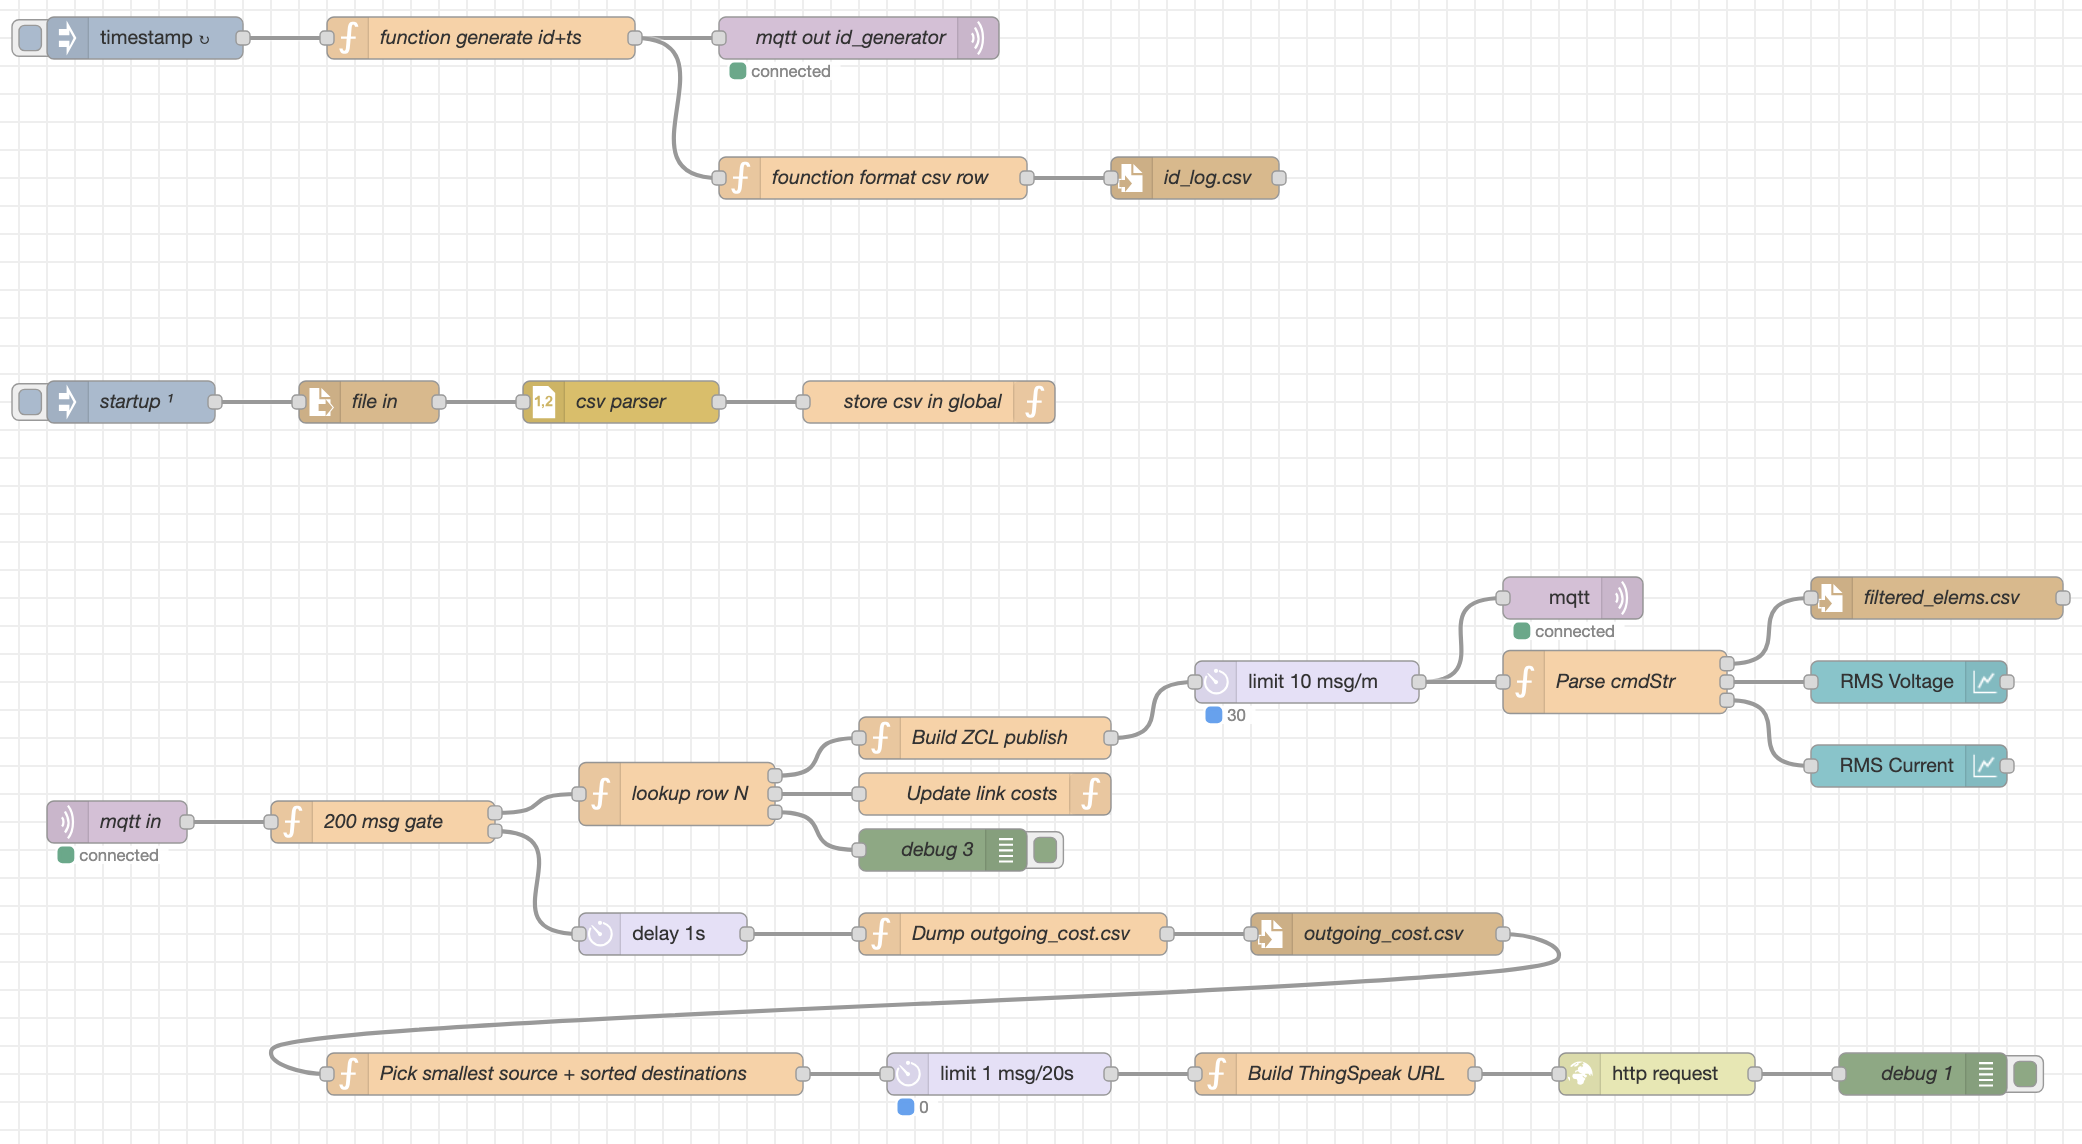
\includegraphics[width=\linewidth]{images/flow_overall.png}
    \caption{Complete Node-RED flow.}
\end{figure}

\textbf{Thingspeak url:} \url{https://thingspeak.mathworks.com/channels/3365849}

\section{Chain A -- Periodic ID Publisher}

Generates a random integer $\mathit{id}\in[0,30000]$ together with the
current UNIX timestamp once per second, publishes the JSON payload to
\texttt{challenge3/id\_generator}, and appends the same fields to
\texttt{id\_log.csv}.

\begin{figure}[h]
    \centering
    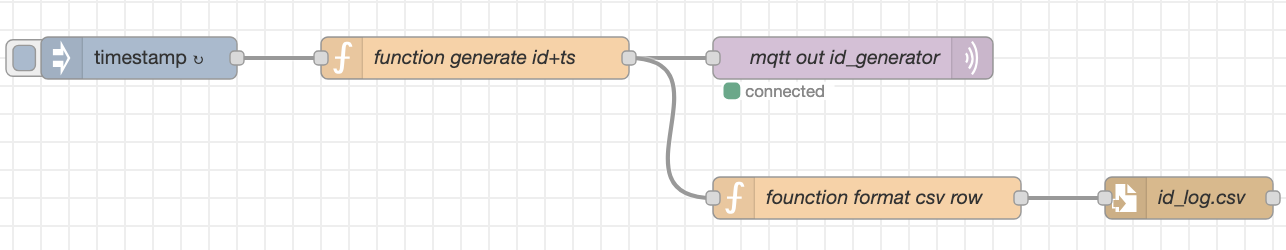
\includegraphics[width=0.85\linewidth]{images/flow_chain_a.png}
    \caption{Chain A -- ID generator and CSV logger.}
\end{figure}

\begin{description}
    \item[timestamp] fires a tick every second.
    \item[function \emph{generate id+ts}] builds the payload
        \verb|{id, timestamp}| as a JavaScript object that Node-RED
        serialises automatically. A flow-context counter stops the
        publisher after exactly 200 ticks, keeping \texttt{id\_log.csv}
        bounded.
        \begin{lstlisting}[caption={Generate ID + timestamp}, label={lst:gen}]
        // Stop publishing after 200 messages
        let pubCount = flow.get('pubCount') || 0;
        if (pubCount >= 200) return null;
        flow.set('pubCount', pubCount + 1);
        
        const id = Math.floor(Math.random() * 30001);
        const timestamp = Math.floor(Date.now() / 1000);
        msg.payload = { id: id, timestamp: timestamp };
        return msg;
        \end{lstlisting}
    \item[mqtt out id\_generator] publishes to topic \texttt{challenge3/id\_generator}
        on \texttt{localhost:1884}.
    \item[function \emph{format csv row}] keeps an incremental row counter
        in the flow context, prepends the header on the first row, and
        emits a newline-terminated CSV line.
        \begin{lstlisting}[caption={Format CSV row}]
        let rowNum = flow.get('idLogRowNum') || 0;
        rowNum++;
        flow.set('idLogRowNum', rowNum);
        
        let line = '';
        if (rowNum === 1) line = 'No.,ID,TIMESTAMP\n';
        line += `${rowNum},${msg.payload.id},${msg.payload.timestamp}\n`;
        
        msg.payload = line;
        return msg;
        \end{lstlisting}
    \item[File (append)] appends each line to \texttt{id\_log.csv}.
\end{description}


\section{Chain B -- CSV Loader (runs once at deploy)}

Loads \texttt{challenge3.csv} into the global context at deploy time so
that downstream chains can look up rows by packet number without
re-reading the file.

\begin{figure}[h]
    \centering
    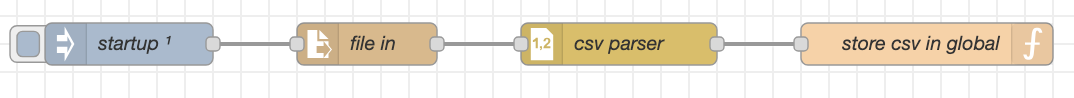
\includegraphics[width=0.85\linewidth]{images/flow_chain_b.png}
    \caption{Chain B -- CSV loader.}
\end{figure}

\begin{description}
    \item[startup (\emph{once on deploy})] fires a single message
        100\,ms after deploy.
    \item[file in] reads the entire \texttt{challenge3.csv} as a UTF-8
        string.
    \item[csv parser] converts the string into an array of row objects
        keyed by the column headers.
    \item[function \emph{store csv in global}] indexes the array by
        \texttt{Packet Number} and stores the resulting dictionary in
        \verb|global.challengeCsv|, providing $O(1)$ lookups.
        \begin{lstlisting}[caption={Store CSV in global}]
        const rows = msg.payload;
        const byPacketNum = {};
        for (const r of rows) {
            byPacketNum[r["Packet Number"]] = r;
        }
        global.set('challengeCsv', byPacketNum);
        node.warn(`Loaded ${rows.length} rows from challenge3.csv`);
        return null;
        \end{lstlisting}
\end{description}

\section{Chain C -- Subscriber, 200-msg Gate and Router}

Subscribes to the same topic, applies a hard cap of 200 processed
messages, computes $N = \mathit{id} \bmod 5218$, retrieves the matching
row from the cached CSV, and dispatches it to one of three
sub-flows (ZCL handler, Link Status handler, or drop).

\begin{figure}[h]
    \centering
    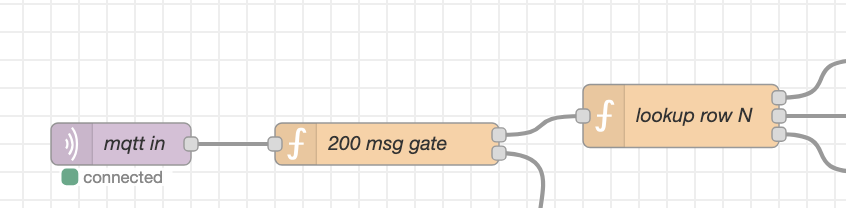
\includegraphics[width=0.95\linewidth]{images/flow_chain_c.png}
    \caption{Chain C -- subscriber, message gate and router.}
\end{figure}

\begin{description}
    \item[MQTT in] subscribes to \texttt{challenge3/id\_generator} with
        \emph{parsed JSON object} output, exposing
        \verb|msg.payload.id| and \verb|msg.payload.timestamp|.
    \item[Function \emph{200-msg gate}] increments a counter on
        \emph{every} arrival; once it reaches 200 a single
        end-of-execution message is emitted on output~2 and all later
        messages are dropped. Ignored messages still consume budget,
        as required.
        \begin{lstlisting}[]
        let count = flow.get('subCount') || 0;
        if (count >= 200) return [null, null];
        
        count++;
        flow.set('subCount', count);
        
        let eof = null;
        if (count === 200) {
            eof = { payload: "end_of_execution" };
            node.warn("Reached 200 messages -- triggering EOF.");
        }
        msg.subCount = count;
        return [msg, eof];
        \end{lstlisting}
    \item[Function \emph{Lookup row N}] computes $N$, fetches
        \verb|global.challengeCsv[N]|, attaches the row, the
        \texttt{SUB\_ID} and the \texttt{Command String} to
        \verb|msg.lookup|, and routes the message to one of three
        outputs by inspecting the Command String for the substrings
        \texttt{ZBEE\_ZCL} or \texttt{Link Status (0x08)}.
        \begin{lstlisting}[]
        const id = msg.payload.id;
        const N = id % 5218;
        const csv = global.get('challengeCsv');
        if (!csv) { node.warn("CSV not loaded yet!"); return null; }
        
        const row = csv[String(N)];
        if (!row) { node.warn(`No row for N=${N}`); return null; }
        
        const cmdStr = row["Command String"] || "";
        msg.lookup = { subId: id, N: N, row: row, cmdStr: cmdStr };
        
        if (cmdStr.includes("ZBEE_ZCL")) { msg.topic = "zcl";  return [msg, null, null]; }
        else if (cmdStr.includes("Link Status (0x08)")) { msg.topic = "linkstatus"; return [null, msg, null]; }
        else { msg.topic = "ignore"; return [null, null, msg]; }
        \end{lstlisting}
\end{description}

\section{Chain D -- ZBEE\_ZCL Handler (output 1 of router)}

Builds the prescribed publish payload, rate-limits it to 10\,msg/min
and publishes it to a topic named after the ZigBee source device. The
same message is parsed for RMS Current / RMS Voltage / Active Power
attributes and forwarded to \texttt{filtered\_elems.csv} and to two
dashboard charts.

\begin{figure}[h]
    \centering
    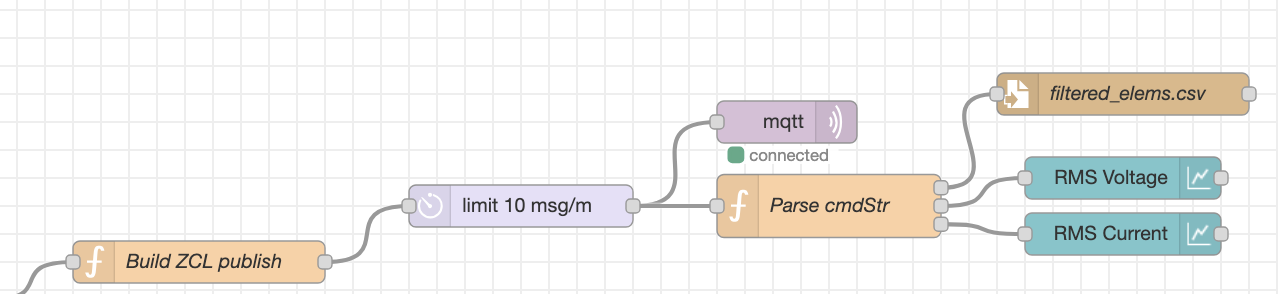
\includegraphics[width=\linewidth]{images/flow_chain_d.png}
    \caption{Chain D -- ZCL publish, filtering and charts.}
\end{figure}

\begin{description}
    \item[Function \emph{Build ZCL publish}] reads the cached row,
        assembles the JSON payload mandated by the specification and
        stores the dynamic topic name (\texttt{Device Name ZigBee
        Source}) in \verb|msg.topic|. The character \texttt{+} is
        stripped from the topic because it is reserved by the MQTT
        protocol as a single-level wildcard and would otherwise be
        rejected by the broker (e.g.\ \texttt{Ledvance Smart+ Plug}).
        \begin{lstlisting}[]
        const lookup = msg.lookup;
        const row = lookup.row;
        const subId = lookup.subId;
        
        const srcAddr     = row["Source Address"];
        const dstAddr     = row["Destination Address"];
        const zbSrcAddr   = row["Source Address ZigBee"];
        const zbDstAddr   = row["Destination Address ZigBee"];
        const zbSrcNameRaw = row["Device Name ZigBee Source"] || "";
        const zbSrcName    = zbSrcNameRaw.replace(/\+/g, "");
        const cmdStr      = row["Command String"] || "";
        
        const payload = {
            timestamp: Math.floor(Date.now() / 1000),
            id: subId,
            "wpan.src": srcAddr,
            "wpan.dst": dstAddr,
            "zbee.src": zbSrcAddr,
            "zbee.dst": zbDstAddr,
            topic: "ZigBee/" + zbSrcName,
            payload: cmdStr
        };
        
        msg.payload = payload;
        msg.topic = zbSrcName;
        return msg;
        \end{lstlisting}
    \item[Delay (\emph{rate limit, 10/min})] queues messages and
        releases at most ten per minute, with no intermediate drops.
    \item[MQTT out (dynamic topic)] empty \emph{Topic} field, so the
        broker uses \verb|msg.topic| at runtime.
    \newpage
    \item[Function \emph{Parse cmdStr}] converts the
        Python-dictionary-style Command String into a JSON object by
        replacing single quotes with double quotes, walks the parallel
        arrays \texttt{Attribute}/\texttt{Status}/\texttt{Data Type} and
        consumes one value at a time from the corresponding typed list
        (\texttt{Int16}, \texttt{Uint16}, \dots) using a per-type
        cursor. Only entries whose attribute is one of the three
        targets \emph{and} for which all of \texttt{Status},
        \texttt{Data Type} and value are populated are retained;
        everything else is discarded, which in practice removes
        \texttt{Read Attributes} \emph{request} packets (no value) and
        spontaneous reports lacking a status. The node has three
        outputs: the CSV chunk, the RMS Voltage chart messages and the
        RMS Current chart messages.
        \begin{lstlisting}[]
        const cmdStr = msg.lookup.cmdStr;

        // Quick reject
        if (!cmdStr.includes("RMS Current") &&
            !cmdStr.includes("RMS Voltage") &&
            !cmdStr.includes("Active Power")) {
            return null;
        }
        
        // Python-dict to JSON
        let obj;
        try {
            obj = JSON.parse(cmdStr.replace(/'/g, '"'));
        } catch (e) {
            node.warn("Parse failed: " + e.message);
            return null;
        }
        // normalize a value to an array
        const arr   = (v) => v === undefined ? [] : Array.isArray(v) ? v : [v];
        // an input like "RMS Voltage (0x0505)" becomes "RMS Voltage"
        const clean = (s) => String(s).replace(/\s*\(0x[0-9a-fA-F]+\)\s*$/, "").trim();
        // extract the leading integer "230 V" becomes "230"
        const num   = (s) => { const m = /^(-?\d+)/.exec(String(s)); return m ? m[1] : String(s); };
        
        const typeMap = {
            "16-Bit Signed Integer":   "Int16",
            "16-Bit Unsigned Integer": "Uint16",
            "8-Bit Signed Integer":    "Int8",
            "8-Bit Unsigned Integer":  "Uint8",
            "32-Bit Signed Integer":   "Int32",
            "32-Bit Unsigned Integer": "Uint32",
        };
        
        const attributes = arr(obj.Attribute);
        const statuses   = arr(obj.Status);
        const dataTypes  = arr(obj["Data Type"]);
        const cursor     = {};
        
        const ts     = msg.payload.timestamp;
        const seqNum = obj["Sequence Number"] || "";
        
        const csvLines = [];
        const voltMsgs = [];
        const currMsgs = [];
        let rowNum = flow.get('filteredRowNum') || 0;
        
        // Walk through every attribute. The values aren't stored
        // alongside their attribute names — they're grouped by data type into
        // separate arrays (Int16, Uint16, etc.). The `cursor` object tracks how
        // many values of each type are already consumed, so on each iteration
        // we pull the *next* value of the matching type.
        for (let i = 0; i < attributes.length; i++) {
            const attrName      = clean(attributes[i]);
            const dataTypeLabel = clean(dataTypes[i] || "");
            const tf            = typeMap[dataTypeLabel];
        
            let value = "";
            if (tf) {
                const list = arr(obj[tf]).map(num);
                const idx  = cursor[tf] || 0;
                value      = list[idx] !== undefined ? list[idx] : "";
                cursor[tf] = idx + 1;
            }
        
            if (attrName !== "Active Power" &&
            attrName !== "RMS Current" &&
            attrName !== "RMS Voltage") continue;
        
            const status   = statuses[i] ? clean(statuses[i]) : "";
            const dtLabel  = clean(dataTypes[i] || "");
        
            if (value === "" || !status || !dtLabel) continue;
        
            rowNum++;
            if (rowNum === 1) {
                csvLines.push("No.,Timestamp,Sequence Number,Attribute,Status,Data Type,Data Value");
            }
            csvLines.push(`${rowNum},${ts},${seqNum},${attrName},${status},${dataTypeLabel},${value}`);
        
            if      (attrName === "RMS Current") currMsgs.push({ payload: Number(value), topic: "RMS Current" });
            else if (attrName === "RMS Voltage") voltMsgs.push({ payload: Number(value), topic: "RMS Voltage" });
        }
        
        flow.set('filteredRowNum', rowNum);
        
        if (csvLines.length === 0) return null;
        
        return [
            { payload: csvLines.join("\n") + "\n" },
            voltMsgs.length ? voltMsgs : null,
            currMsgs.length ? currMsgs : null
        ];
        \end{lstlisting}
    \item[File (append)] writes the CSV chunk to
        \texttt{filtered\_elems.csv}.
    \item[Chart \emph{RMS Voltage} / \emph{RMS Current}] two
        node-red-dashboard line charts on the same UI group.
\end{description}

\begin{figure}[h]
    \centering
    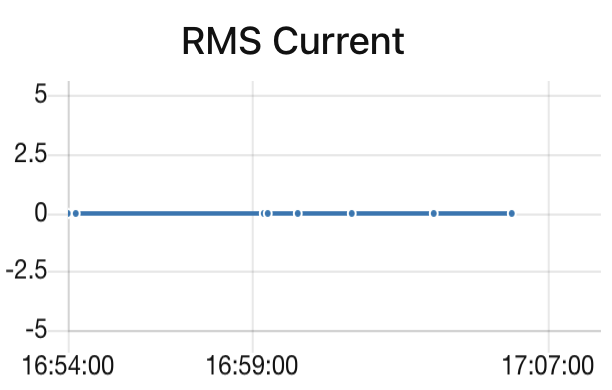
\includegraphics[width=0.45\linewidth]{images/chart_rms_current.png}
    \hfill
    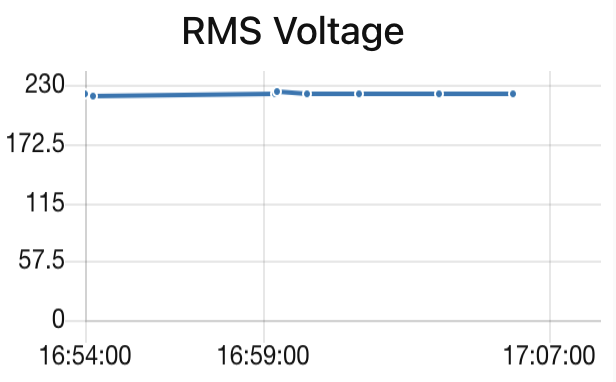
\includegraphics[width=0.45\linewidth]{images/chart_rms_voltage.png}
    \caption{Live charts of RMS Current and RMS Voltage.}
\end{figure}

\section{Chain E -- Link Status Handler, Flush and ThingSpeak}

Maintains an ordered list of outgoing link costs, keyed by
$(\text{ZigBee source}, \text{destination})$ pairs. Rows are appended
in the order Link Status messages are processed; when a pair is seen
again, its cost is updated \emph{in place} so that the row preserves
its original sequence number. Once the 200-message budget is
exhausted, the list is flushed to \texttt{outgoing\_cost.csv} in
processing order, and the smallest source's destinations are then
sorted hexadecimally and streamed to a public ThingSpeak channel at
one update every 20\,s.

\begin{figure}[h]
    \centering
    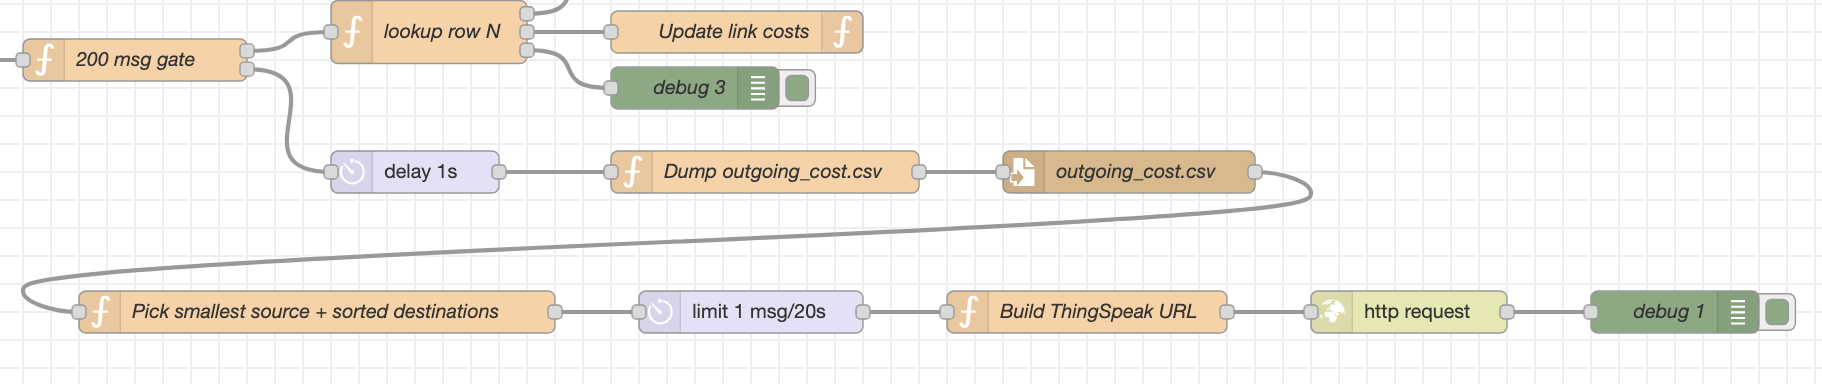
\includegraphics[width=\linewidth]{images/flow_chain_e.png}
    \caption{Chain E -- Link Status update, end-of-run flush and ThingSpeak publisher.}
\end{figure}

\begin{description}
    \item[Function \emph{Update link costs}] (wired to router output~2)
        parses the Command String and iterates the \texttt{Links}
        array. Two data structures are maintained in the global
        context: an ordered \verb|linkRows| array (the rows that will
        ultimately be written to disk, in processing order) and an
        index \verb|linkRowIdx| mapping the key
        \texttt{"src|dst"} to its position in the array. A new
        $(\text{src},\text{dst})$ pair is appended; a repeated pair has
        only its cost updated in place, leaving its row number
        unchanged, as recommended in the clarifications.
        \begin{lstlisting}[]
        const row    = msg.lookup.row;
        const cmdStr = msg.lookup.cmdStr;
        
        const source = String(row["Source Address ZigBee"] || "").trim().toLowerCase();
        if (!source.startsWith("0x")) return null;
        
        let obj;
        try { obj = JSON.parse(cmdStr.replace(/'/g, '"')); }
        catch (e) { node.warn("Link Status parse failed: " + e.message); return null; }
        
        const links = obj.Links;
        if (!Array.isArray(links)) return null;
        
        let rows = global.get('linkRows')   || [];
        let idx  = global.get('linkRowIdx') || {};
        
        for (const link of links) {
            const dest = String(link.Address || "").trim().toLowerCase();
            const cost = parseInt(link["Outgoing Cost"], 10);
            if (!dest.startsWith("0x") || isNaN(cost)) continue;
        
            const key = source + "|" + dest;
            if (idx[key] !== undefined) {
                rows[idx[key]].cost = cost;
            } else {
                idx[key] = rows.length;
                rows.push({ src: source, dst: dest, cost: cost });
            }
        }
        global.set('linkRows', rows);
        global.set('linkRowIdx', idx);
        return null;
        \end{lstlisting}
    \item[Delay (\emph{1\,s})] introduced after the gate's EOF output
        to let the 200th message finish propagating through chain~D
        and the link-cost updater before the flush starts.
    \item[Function \emph{Dump outgoing\_cost.csv}] guarded by a
        single-shot flag, iterates the \verb|linkRows| array in its
        natural (processing) order and emits one CSV row per entry,
        with an incremental \texttt{No.}\ field. No sorting is applied
        at this stage.
        \begin{lstlisting}[]
        if (flow.get('flushed')) return null;
        flow.set('flushed', true);
        
        const rows = global.get('linkRows') || [];
        const lines = ["No.,Source,Destination,Cost"];
        for (let i = 0; i < rows.length; i++) {
            const r = rows[i];
            lines.push(`${i+1},${r.src},${r.dst},${r.cost}`);
        }
        
        node.warn(`Flushed ${rows.length} link entries.`);
        msg.payload = lines.join("\n") + "\n";
        return msg;
        \end{lstlisting}
    \item[File (overwrite)] writes the resulting CSV to
        \texttt{outgoing\_cost.csv}.
    \item[Function \emph{Pick smallest source}] inspects the
        \verb|linkRows| array, derives the unique set of sources,
        selects the hexadecimally smallest one (typically
        \texttt{0x0000}), filters its rows and sorts them by
        destination address in ascending hexadecimal order. One
        message per destination is emitted downstream, carrying the
        corresponding outgoing cost.
        \begin{lstlisting}[]
        const rows = global.get('linkRows') || [];
        if (rows.length === 0) return null;
        
        const hexCmp = (a, b) => parseInt(a, 16) - parseInt(b, 16);
        const sources  = [...new Set(rows.map(r => r.src))].sort(hexCmp);
        const smallest = sources[0];
        
        const smallestRows = rows
            .filter(r => r.src === smallest)
            .sort((a, b) => hexCmp(a.dst, b.dst));
        
        node.warn(`Smallest source = ${smallest}, ${smallestRows.length} destinations.`);
        return [smallestRows.map(r => ({
            payload: { source: smallest, destination: r.dst, cost: r.cost }
        }))];
        \end{lstlisting}


    \item[Delay (\emph{rate limit, 1 / 20\,s})] enforces the ThingSpeak
        rate limit.
    \item[Function \emph{Build ThingSpeak URL}] constructs the URL\\
        \verb|https://api.thingspeak.com/update?api_key=<KEY>&field1=<cost>|\\
        and stores it in \verb|msg.url|.
        \begin{lstlisting}[]
        const API_KEY = "SECRET";
        msg.url = `https://api.thingspeak.com/update?api_key=${API_KEY}&field1=${msg.payload.cost}`;
        msg.method = "GET";
        node.warn(`ThingSpeak: dst=${msg.payload.destination} cost=${msg.payload.cost}`);
        return msg;
        \end{lstlisting}
    \item[HTTP request] performs the API call.
\end{description}

\section{Deliverables}
\label{sec:deliverables}

\begin{itemize}
    \item Node-RED flow export: \texttt{nodered.json}
    \item CSV files: \texttt{id\_log.csv}, \texttt{filtered\_elems.csv},
          \texttt{outgoing\_cost.csv}
    \item ThingSpeak channel (public):
          \url{https://thingspeak.mathworks.com/channels/3365849}
\end{itemize}
\begin{figure}[h]
    \centering
    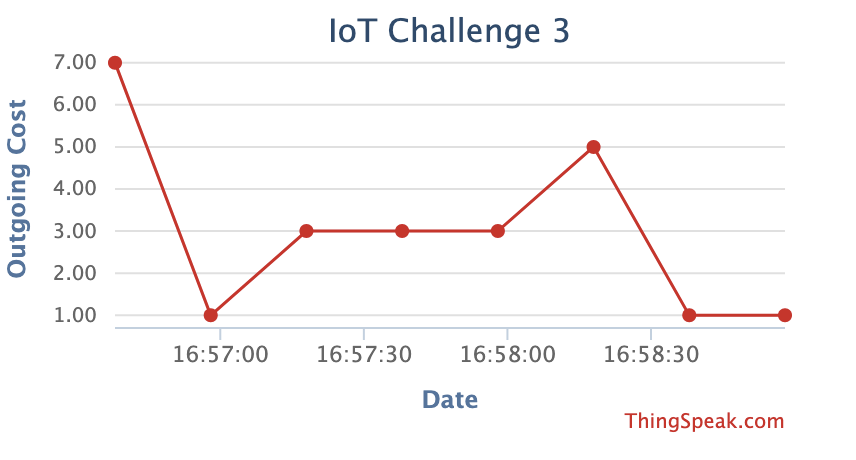
\includegraphics[width=\linewidth]{images/thingspeak_graph.png}
\end{figure}

\end{document}
